
\subsection{Batch Processing using "batch macro" function}
In above macro, list of functions were wrapped inside macro "title"\{ code \} 
so that these macro functions could be executed by single command from menu. 
To apply such a sequence of macro functions for many images in a single folder 
(say you have one-thousand images you want to contrast enhance and also to Gaussian-blur), 
there are two ways. One way is to further extend the macro by adding file-accessing macro functions and 
looping those functions (you will learn this later). 
Another way is to do such "batch processing" by copy and pasting list of
macro functions to batch-processing interface. 
This interface could be used by \ijmenu{[Process -> Batch -> Macro]}

\begin{figure}[htbp]
\begin{center}
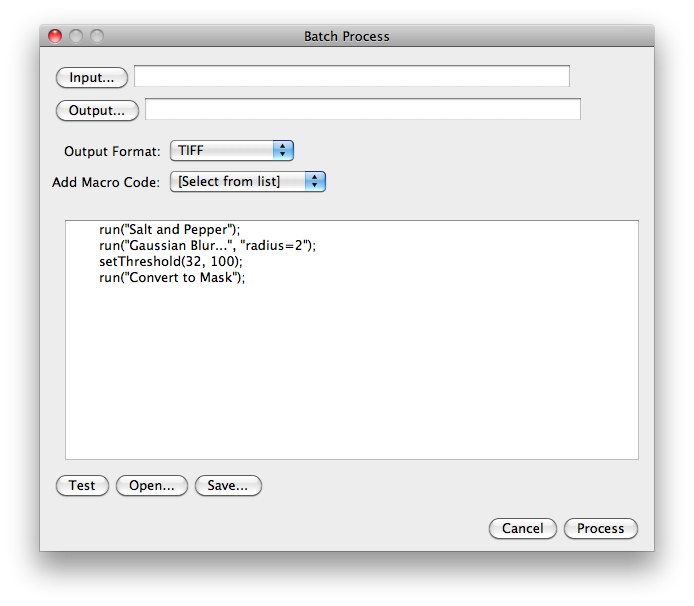
\includegraphics[scale=0.4]{fig/BatchProcessing.png}
\caption{Batch Processing Dialog} \label{fig_BatchProcessInterface}
\end{center}
\end{figure}

In "Input" field, select the folder where image files are stored. 
In output field, select a destination folder where processed images will be stored. 
You then copy and paste the list of macro functions in the code field such as 
shown in Fig. \ref{fig_BatchProcessInterface}. 
In the case shown in this figure, line 6 to 9 was copied and pasted. 
Clicking "Process" button will start the processing.
\newpage

